\documentclass[12pt,letterpaper]{article}

\usepackage{amsmath, amsthm}
\usepackage{microtype, parskip}
\usepackage[comma,numbers,sort&compress]{natbib}
\usepackage{lineno}
\usepackage{docmute}
\usepackage{caption, subcaption, multirow, morefloats, rotating}
\usepackage{wrapfig}

\frenchspacing

\begin{document}
\section{Methods}

\subsection{Fossil occurrence information}

The dataset analyzed here is derived from the a combination of the occurrence information from \citet{Miller2009a} and the body size data from \citet{Payne2014}. The \citet{Miller2009a} dataset is based on the Paleobiology Database (http://www.paleodb.org); see \citet{Miller2009a} for a full description of the inclusion criterion. 

Sampled occurrences were restricted to those with latitude and longitude coordinates, assignment to either epicontinental or open-ocean environment, and being of a genus present in the body size dataset. Genus duration was calculated as the number of geologic stages from first appearance to last appearance, inclusive. Genera who's last appearance was in a stage preceding a mass extinction were right censored, and genera with a duration of only one stage and were left censored (see below for explanation of censoring). The covariates used to model genus duration were geographic range size (\(r\)), environmental preference (\(v\)), and body size (\(m\)). 

Geographic range was calculated using an occupancy approach. First, all occurrences were projected onto an equal-area cylindrical map projection. Each occurrence was then assigned to one of the cells of a 70 \(\times\) 34 regular raster grid placed on the map. Each grid cell represents approximately 250,000 km\(^{2}\). Following this, for each stage, the total number of grid cells occupied is calculated. The number of grid cells that each genus present occurs in was then calculated and made relative by dividing by the total number of possible cells. Finally, mean relative genus occupancy was calculated as the mean of per stage relative occupancy.

Body size data was sourced directly from \citet{Payne2014}. Because those measurements are presented with out quantified error, a measurement error model similar to the one for environmental affinity could not be implemented.

Prior to analysis some covariates were transformed in order to improve interpretation. Geographic range size, which can only have between 0 and 1, was logit transformed. Body size, which is defined for all positive real values was natural log transformed. These covariates were then standardized by mean centering and dividing by two times their standard deviation following \citet{Gelman2007}.

\subsubsection{Uncertainty in environmental preference}
The calculation and inclusion of environmental affinity in the subsequent survival model is a statistical procedure that takes into account our uncertainty based on where fossils tend to occur. Because we cannot directly observe if a fossil taxon had occurrences restricted to only a single environmental, instead we can only get an of affinity with some amount of uncertainty. One advantage of using a Bayesian analytical context is that both parameters and data are considered random samples from some underlying distribution, which means it is possible to model the uncertainty in our covariates of interest \citep{Gelman2013d}. In this case, this is the genus affnity to either epicontiental settings or not. This approach is conceptually similar to \citet{Simpson2009} but instead of obtaining a single point estimate, an entire posterior distribution is estimated.

The first step is to determine the probability \(\theta\) at which genus \(i\) occurs in an epicontinental settings based on its own pattern of occurrences. Define \(e_{i}\) as the number of occurrences of genus \(i\) in an epicontiental sea and \(o_{i}\) as the number of occurrences of genus \(i\) not in an epicontinental sea (e.g. open ocean). Because the value of inters is the probability of occurring in an epicontinental environment, given the observed fossil record, I assume that probability follows a beta distribution. We can then define our sampling statement as
\begin{equation}
  e_{i} \sim \mathrm{Binomial}(e_{i} + o_{i}, \theta_{i}).
  \label{eq:epi_lik}
\end{equation}
I used a flat prior of \(\theta_{i}\) defined as \(\theta_{i} \sim \mathrm{Beta}(1, 1)\). Because the beta distribution is the conjugate prior for the binomial distribution, the posterior is easy to compute in closed form. The posterior probability of \(\theta\) is then 
\begin{equation}
  \theta_{i} \sim \mathrm{Beta}(e_{i} + 1, o_{i} + 1)
  \label{eq:epi_post}
\end{equation}

It is extremely important, however, to take into account the overall environmental occurrence probability of all other genera present at the same time as genus \(i\). This is incorporated as an additional probability \(\Theta\). Define \(E_{i}\) as the total number of other fossil occurrences (e.g. excepting for genus \(i\)) in epicontinental seas during stages where \(i\) occurs and \(O_{i}\) as the number of other fossil occurrences not on epicontinental seas. We can then define the sampling statement as
\begin{equation}
  E_{i} \sim \mathrm{Binomial}(E_{i} + O_{i}, \Theta_{i}).
  \label{eq:bck_lik}
\end{equation}
Again, I used a flat prior of \(\Theta_{i}\) defined as \(\Theta_{i} \sim \mathrm{Beta}(1, 1)\). The posterior of \(\Theta\) is then simply defined as
\begin{equation}
  \Theta_{i} \sim \mathrm{Beta}(E_{i} + 1, O_{i} + 1)
  \label{eq:bck_post}
\end{equation}

I then define the environmental affinity of genus \(i\) as \(v_{i} = \theta_{i} - \Theta_{i}\). \(v_{i}\) is a value that can range between -1 and 1, where negative values indicate that genus \(i\) tends to occur in open ocean environments while positive values indicate that genus \(i\) tends to occur in epicontiental environments.

While this approach is noticeably more complicated than previous ones \citep{Foote2006,Miller2001,Simpson2009,Kiessling2007a} there are some important benefits to both using a continuous measure of affinity as well directly modeling our uncertainty. In order to show case some of these benefits, I performed a simulation analysis of how modal/maximum \textit{a posteriori}(MAP) estimates versus full posterior estimates.

In this simulation, I first defined the ``background'' epicontinental occurrence \(\theta_{b}\) as 0.50 with a small amount of noise. This was represented as a beta distribution 
\begin{equation}
  \theta_{b} = \mathrm{Beta}(\alpha = 2500, \beta = 2500). 
  \label{eq:bck_sim}
\end{equation}
This choice of parameters for the distribution reflects the average number of background occurrences for either epicontinental or open ocean environments per genus.

Using this background occurrence ratio, randomly generated the occurrence patterns 1000 simulated taxa. This was done at multiple sample sizes (1, 2, 3, 4, 5, 10, 25, 50, 100) in order to demonstrate the effects of increasing sample size on the confidence of environmental affinity. For each simulated taxon I calculated the full posterior distribution while assuming a flat Beta prior (\(\mathrm{Beta}(1, 1)\)). Using the full posterior I calculated the MAP probability of occurring in epicontinental environments. The environmental affinity was calculated for each of the simulated taxa using both the full posterior and the MAP estimate. In this toy example, environmental affinity can range between -0.5 and 0.5.

As should be expected, as sample size increases the distribution of MAP estimates converge on the true value (Fig. \ref{fig:env_mode}). For taxa with less than 10 occurrences, the MAP estimate is biased towards over estimates of affinity. Note that the mode of the beta distirbution is not defined for situations where there were 0 draws of one of the environmental conditions. Instead, the vertical line is based entirely on the observed occurrences. 
\begin{figure}[ht]
  \centering
  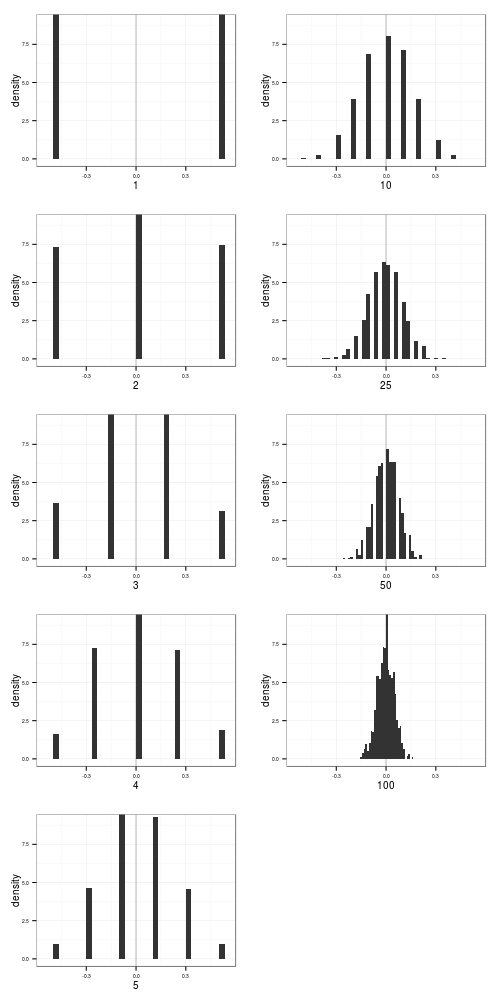
\includegraphics[height = \textheight,width=\textwidth,keepaspectratio=true]{figure/env_mode_dist}
  \caption{<+caption text+>}
  \label{fig:env_mode}
\end{figure}

In contrast, we can compare the true occurrence probability distribution versus the posterior estimate for a given sample (Fig. \ref{fig:env_post}). When sample sizes are low, posterior estimates are flat and represent a compromise between the likelihood (equivalent to MAP) and the flat prior. Because of this, estimates from small sizes are less likely to be overly biased. This is further emphasized by inspection of the estimates of environmental affinity for the simulated taxa (Fig. \ref{fig:env_diff}). Posterior estimates from simulated taxa with small sample size have a much broader distribution that both allows for the extreme observation but still captures the ``true'' value (0). 
\begin{figure}[ht]
  \centering
  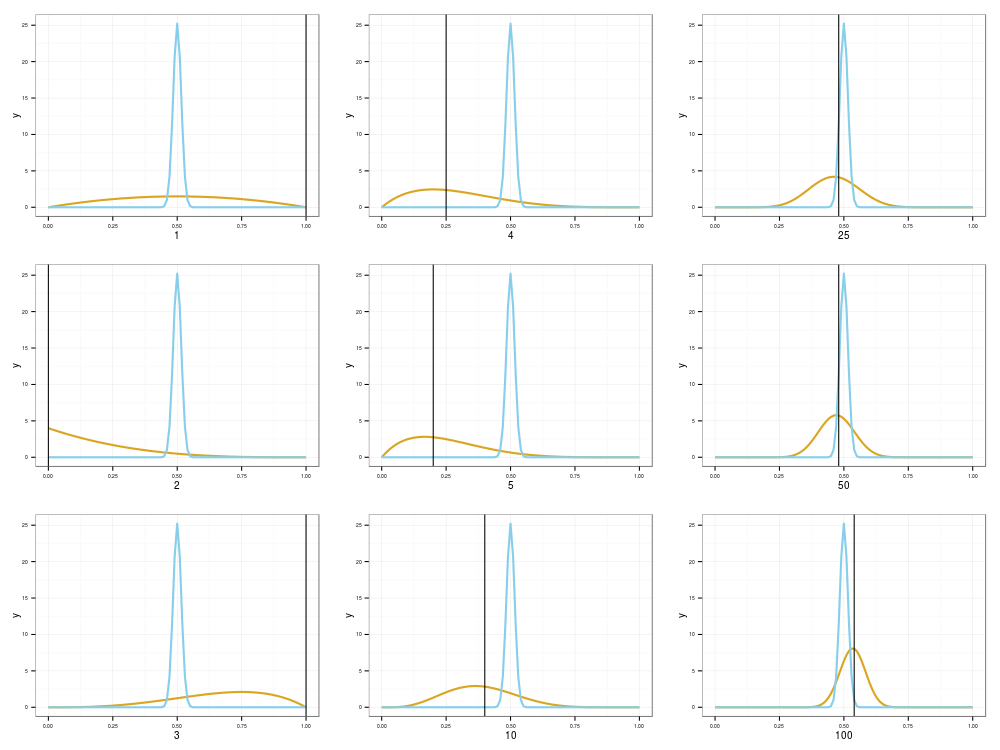
\includegraphics[height = \textheight,width=\textwidth,keepaspectratio=true]{figure/env_post_inspect}
  \caption{<+caption text+>}
  \label{fig:env_post}
\end{figure}

\begin{figure}[ht]
  \centering
  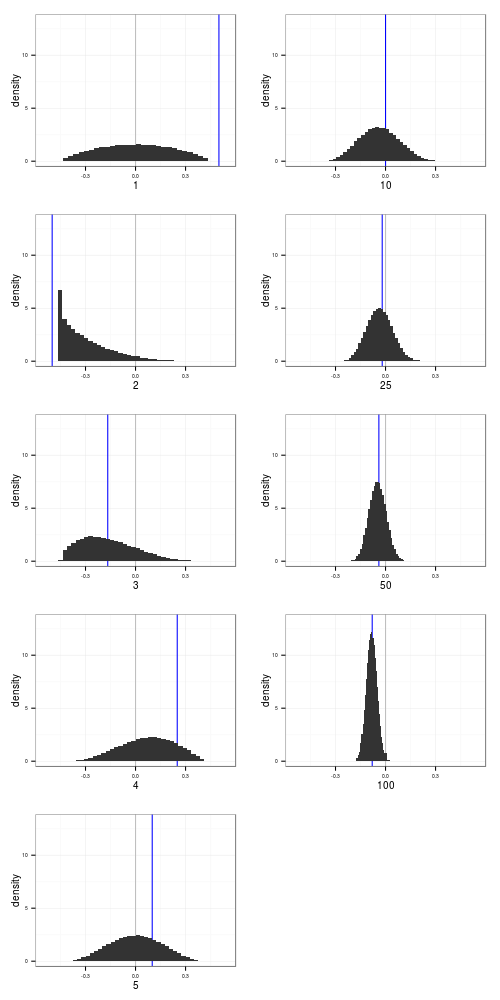
\includegraphics[height = \textheight,width=\textwidth,keepaspectratio=true]{figure/env_diff}
  \caption{<+caption text+>}
  \label{fig:env_diff}
\end{figure}

By defining environmental preference as the difference in full posterior estimates of occurrence probability, it is possible to include taxa with low sample sizes that are normal discarded \citep{Foote2006,Miller2001,Simpson2009,Kiessling2007a}. Additionally, 55+\% of observed Paleozoic brachiopod genera have less than 10 occurrences which is the sample size range where MAP (or ML) estimates would be most biased.
This is preferable to the difference in MAP estimates, especially for taxa with small sample sizes (blue line; Fig. \ref{fig:env_diff}).


% behavior of MAP estimates
%   as sample size increases, converge on true (10+)
% behavior of posterior
%   compromise between likelihood of data occurrences and (flat) prior
%   really important for small sample sizes
%   at 10+ makes no difference anymore
%   this is also kind obvious from the estimates of \(v\)
% how many taxa have less than 10 occurrences? \approx 55\%

\subsection{Survival model}

Genus durations were modeled in a Bayesian parameteric survival analysis framework. Durations were assumed to follow either an exponential or Weibull distribution. Each of these distributions makes strong assumptions about how duration may effect extinction risk. Use of the exponential distribution assumes that extinction risk is independent of duration. In contrast, use of the Weibull distribution allows for age dependent extinction via the shape parameter \(\alpha\), though only as a monotonic function of duration. Importantly, the Weibull distribution is equivalent to the exponential distribution when \(\alpha = 1\). In general, the notation used here follows \citet{Gelman2007}, \citet{Gelman2013d}, and \uppercase{stan manual}.

The simplest model of genus duration includes no covariate or structural information. Define \(y_{i}\) as the duration in stages of genus \(i\), where \(i = 1, \dots, n\) and \(n\) is the number of observed genera. These two models are them simply defined as
\begin{equation}
  \begin{aligned}
    y_{i} &\sim \mathrm{Exponential}(\lambda) \\
    y_{i} &\sim \mathrm{Weibull}(\alpha, \sigma).
  \end{aligned}
  \label{eq:simple}
\end{equation}
Note that \(\lambda\) is a ``rate'' or inverse-scale while \(\sigma\) is a scale parameter, meaning that \(\frac{1}{\lambda} = \sigma\).

These simple models can then be expanded to include covariate information as predictors by reparameterizing \(\lambda\) and \(\sigma\) as a regression \citep{Klein2003}. Each of the covariates of interest is given its own regression coefficient (e.g. \(\beta_{range}\)) along with an intercept term \(\beta_{0}\). There are some additional complications to the parameterization of \(\sigma\) associated with the inclusion of \(\alpha\) as well as interpretability \citep{Klein2003}. Both of these cases are written more fully as
\begin{equation}
  \begin{aligned}
    \lambda_{i} &= \exp(\beta_{0} + \beta_{r} r_{i} + \beta_{v} v_{i} + \beta_{v^{2}} v_{i}^{2} + \beta_{m} m_{i}) \\
    \sigma_{i} &= \exp\left(\frac{-(\beta_{0} + \beta_{r} r_{i} + \beta_{v} v_{i} + \beta_{v^{2}} v_{i}^{2} + \beta_{m} m_{i})}{\alpha}\right).
  \end{aligned}
  \label{eq:regression}
\end{equation}
The regression equations are exponentiated because both \(\lambda\) and \(\sigma\) are only defined for positive reals. The quadratic term for environmental affinity \(v\) is to allow for the possiblity of a nonlinear relationship between environmental affinity and extinction risk.

The models which incorporate both equations \ref{eq:simple} and \ref{eq:regression} can then be further expanded to allow all of the \(\beta\) coefficients, including \(\beta_{0}\), to vary with origination cohort while also modeling their covariance and correlation. This is called a varying-intercepts, varying-slopes model \citep{Gelman2007}. It is much easier to represent and explain how this is parameterized using matrix notation. First, define \(\mathbf{B}\) as \(k \times J\) matrix of the \(k\) coefficients including the intercept term (\(k = 5\)) for each of the \(J\) cohorts. Second, define \(\mathbf{X}\) as a \(n \times k\) matrix where each column is one of the covariates of interest. Importantly, \(\mathbf{X}\) includes a columns of all 1s which correspond to the constant term \(\beta_{0}\). Third, define \(j[i]\) as the origination cohort of genus \(i\), where \(j = 1, \dots, J\) and \(J\) is the total number of observed cohorts.

Using the above hierarchical expansion to the model, we then rewrite \(\lambda\) and \(\sigma\) in matrix notation as
\begin{equation}
  \begin{aligned}
    \lambda_{i} &= \exp(\mathbf{X}_{i} \mathbf{B}_{j[i]}) \\
    \sigma_{i} &= \exp\left(\frac{-(\mathbf{X}_{i} \mathbf{B}_{j[i]})}{\alpha}\right). 
  \end{aligned}
  \label{eq:multivariate}
\end{equation}

At face value, the above parameterization (Eq. \ref{eq:multivariate}) is opaque as to how the covariance and correlation between elements of \(\mathbf{B}\) are estimated. This becomes more apparent after defining the prior distribution of \(\mathbf{B}\). Because \(\mathbf{B}\) is a matrix, I used a multivariate normal prior with unknown vector of means \(\mu\) and covariance matrix \(\mathbf{\Sigma}\). This is written as 
\begin{equation}
  \mathbf{B} \sim \mathrm{MVN}(\mu_{\mathbf{B}}, \Sigma_{\mathbf{B}}).
  \label{eq:beta_prior}
\end{equation}
\(\mu_{\mathbf{B}}\) is length \(k\) vector representing the overall mean of the distributions of \(\beta\) coefficients. \(\Sigma_{\mathbf{B}}\) is a \(k \times k\) covariance matrix of the \(\beta\) coefficients.

What remains is assigning priors the elements of \(\mu_{\mathbf{B}}\) and the covariance matrix \(\Sigma_{\mathbf{B}}\). Each of the elements of vector \(\mu_{\mathbf{B}}\) were given independent, weakly-informative normal priors. The prior for \(\Sigma_{\mathbf{B}}\) is a bit more complicated. While the conjugate prior distribution for a covariance matrix is the inverse-Wishart \citep{Gelman2013d}, because I am using a variant for Hamiltonian Monte Carlo (HMC) called No U-Turn Sampling (NUTS) for posterior estimation as opposed to Gibbs sampling there is not benefit for using a conjugate prior \uppercase{stan manual}. Additionally, the inverse-Wishart distribution strongly constraints the off-diagonal elements of the covariance matrix. Instead, it is better to model the correlation matrix and separate variance terms for each of the \(k\) coefficients. This is possible because of the relationship between a covariance and a correlation matrix, defined as 
\begin{equation}
  \Sigma_{\mathbf{B}} = \text{Diag}(\tau_{B}) \Omega_{\mathbf{B}} \text{Diag}(\tau_{B})
  \label{eq:covcor}
\end{equation}
where \(\tau_{B}\) is a length \(k\) vector of variances and Diag(\(\tau_{B}\)) is a diagonal matrix.

I used a LKJ prior distribution for \(\Omega_{\mathbf{B}}\) as recommended by \uppercase{stan manual}. An LKJ is a single parameter multivariate distribution where values of \(\eta\) greater than 1 concentrate density at the unit correlation matrix, which corresponds to no correlation between the \(\beta\) coefficients. The scale parameter, \(\tau_{B}\), is given a weakly informative half-Cauchy (C\(^{+}\)) prior following \citet{Gelman2006a}.

Given all the above, the exponential distribution based model is then defined, including priors, as 
\begin{equation}
  \begin{aligned}
    y_{i} &\sim \mathrm{Exponential}(\lambda) \\
    \lambda_{i} &= \exp(\mathbf{X}_{i} \mathbf{B}_{j[i]}) \\
    \mathbf{B} &\sim \mathrm{MVN}(\mu_{\mathbf{B}}, \Sigma_{\mathbf{B}}) \\
    \Sigma_{\mathbf{B}} &= \text{Diag}(\tau_{B}) \Omega_{\mathbf{B}} \text{Diag}(\tau_{B}) \\
    \mu_{\kappa} &\sim \mathcal{N}(0, 5) \text{ for } \kappa \in 1:k \\
    \tau_{\kappa} &\sim \mathrm{C^{+}}(1) \text{ for } \kappa \in 1:k \\
    \Omega &\sim \text{LKJ}(2).
  \end{aligned}
  \label{eq:exp_total}
\end{equation}
The Weibull distribution based model is then also defined as
\begin{equation}
  \begin{aligned}
    y_{i} &\sim \mathrm{Weibull}(\alpha, \sigma) \\
    \sigma_{i} &= \exp\left(\frac{-(\mathbf{X}_{i} \mathbf{B}_{j[i]})}{\alpha}\right) \\
    \mathbf{B} &\sim \mathrm{MVN}(\mu_{\mathbf{B}}, \Sigma_{\mathbf{B}}) \\
    \Sigma_{\mathbf{B}} &= \text{Diag}(\tau_{B}) \Omega_{\mathbf{B}} \text{Diag}(\tau_{B}) \\
    \alpha &\sim \mathrm{C^{+}}(2) \\
    \mu_{\kappa} &\sim \mathcal{N}(0, 5) \text{ for } \kappa \in 1:k \\
    \tau_{\kappa} &\sim \mathrm{C^{+}}(1) \text{ for } \kappa \in 1:k \\
    \Omega &\sim \text{LKJ}(2).
  \end{aligned}
  \label{eq:wei_total}
\end{equation}
Note that the above formulations of each model (Eq. \ref{eq:exp_total}, \ref{eq:wei_total}) does not include how the uncertainty in environmental affinity is included nor how censored observations are included. An explination of including censored observations follows.


\subsection{Censored observations}
A key aspect of survival analysis is the inclusion of censored, or incompletely observed, data points \citep{Ibrahim2001,Klein2003}. The two classes of censored observations encountered in this study were right and left censored observations. Right censored genera are those that did not go extinct during the window of observation, or genera that are still extant. Left censored observations are those taxa that it is only known when it was extinct by. To put another way, this is a taxon that went extinct but the observed duration is an over estimate of the actual duration. 

In the context of this study, I considered all genera that had a duration of only one geologic stage to be left censored as we do not have a finer degree of resolution. Conceptually, this is similar to if I was studying, say, survival patterns in rats and an individual had died between the start of the experiment and next time the rats were observed. We know the rat lived no more than day.

The key function for modeling censored observations is the survival function, or \(S(t)\). \(S(t)\) corresponds to the probability that a genus having existed for \(t\) stages will not have gone extinct while \(h(t)\) corresponds to the instantaneous extinction rate at taxon age \(t\) \cite{Klein2003}. For an exponential model, \(S(t)\) is defined as
\begin{equation}
  S(t) = \exp(-\lambda t),
  \label{eq:exp_surv}
\end{equation}
and for the Weibull distribution \(S(t)\) is defined as
\begin{equation}
  S(t) = \exp\left(-\left(\frac{t}{\sigma}\right)^{\alpha}\right).
  \label{eq:wei_surv}
\end{equation}
\(S(t)\) is equivalent to the complementary cumulative distribution function, \(1 - F(t)\) \citep{Klein2003}. 

For right censored observations, instead of calculating the likelihood as normal (Eq. \ref{eq:multivariate}) the likelihood of an observation is evaluated using \(S(t)\). Conceptually, this approach calculates the likelihood of observing a taxon that existed for at least that long. For left censored data, instead the likelihood is calculated using \(1 - S(t)\) which corresponds to the likelihood of observing a taxon that existed no longer than \(t\).

The full likelihood statements incorporating fully observed, right censored, and left censored observations are then
\begin{equation}
  \begin{aligned}
    \mathcal{L} &\propto \prod_{i \in C} \mathrm{Exponential}(y_{i} | \lambda) \prod_{j \in R} S(y_{j} | \lambda) \prod_{k \in L} \left(1 - S(y_{k} | \lambda)\right) \\
    \mathcal{L} &\propto \prod_{i \in C} \mathrm{Weibull}(y_{i} | \alpha, \sigma) \prod_{j \in R} S(y_{j} | \alpha, \sigma) \prod_{k \in L} \left(1 - S(y_{k} | \alpha, \sigma)\right)
  \end{aligned}
  \label{eq:censored_likelihood}
\end{equation}
where \(C\) is the set of all fully observed taxa, \(R\) the set of all right censored taxa, and \(L\) the set of all left-censored taxa.


\subsection{Parameter estimation}
Given the above likelihood and prior statements, the posterior probabilities of all parameters was approximated using a Markov-chain Monte Carlo routine using a variant of Hamiltonian Monte Carlo called the No-U-Turn Sampler \citep{Hoffman2014} as implemented in the probabilistic programming language Stan \citep{stan-software:2014}. The estimate of the posterior distribution were approximated from four parallel chains run for 10000 draws split half warm-up and half sampling thinned to every 10 sample for a total of 5000 samples. Chain convergence was assessed via the scale reduction factor \(\hat{R}\) where values close to 1 (\(\hat{R} < 1.1\)) indicate approximate convergence. Convergence means that the chains are approximately stationary and the samples are well mixed \citep{Gelman2013d}.


\subsection{Model evaluation}

Models were evaluated using both a series of multiple posterior predictive checks and an estimate of out-of-sample predictive accuracy. 

The motivation behind posterior predictive checks as tools for determining model adequacy is that replicated data sets using the fitted model should be similar to the original data \citep{Gelman2013d}. Systematic differences between the simulations and observed indicate weaknesses of the currently fit model. An example of a technique that is very similar would be inspecting the residuals and Q-Q plots from a linear regression.

The strategy behind posterior predictive checks is to draw simulated values from the joint posterior predictive distribution, \(p(y^{rep} | y)\), and then compared to the original observed values \citep{Gelman2013d}. To accomplish this, for each replicate, a single value is drawn from the marginal posterior distributions of each regression coefficient from the final model (Eq. \ref{eq:exp_total}, \ref{eq:wei_total}). Then, given the covariate information for each of the observations \(\mathbf{X}\), a new set of \(n\) genus durations are generated giving a single replicated data set \(y^{rep}\). This is repeated 1000 times in order to provide a distribution of possible values that could have been observed given the model. 

In order to compare the fitted model to the observed data, various graphical comparisons or test quantities need to be defined. The principal comparison used here is a comparison between non-parameteric approximation of the survival function \(S(t)\) as estimated from both the observed data and each of the replicated data sets. The purpose of this comparison is to determine if the model approximates the same survival/extinction pattern as the original data. 

I also did a graphical examination of the deviance residuals. While normal residuals are defined as \(y_{i}^{rep} - y_{i}\), deviance residuals are a specific class of residuals derived with non-normal errors in mind. The definition of deviance residuals for a Weibull regression, of which the above models can be considered, is as follows. First define the cumulative hazard function \(\Lambda(t)\) for the Weibull distribution \citep{Klein2003}. Given \(S(t)\) (Eq. \ref{eq:wei_surv}), the cumulative hazard function is 
\begin{equation}
  \Lambda(t) = -log\left(S\left(t\right)\right).
\end{equation}

Next, define martingale residuals \(m\) as
\begin{equation}
  m_{i} = I_{i} - \Lambda(t_i).
\end{equation}
\(I\), called the inclusion vector, is vector of length \(n\) where \(I_{i} = 1\) means the observation is completely observed and \(I_{i} = 0\) means the observation is censored. Martingale residuals have a mean of 0, range between 1 and \(-\infty\), and can be viewed as the difference between the observed number of deaths between 0 and \(t_{i}\) and the expected number of deaths based on the model. However, martingale residuals are asymmetrically distributed, and can not be interpreted in the same manner as standard residuals. 

The solution to this is to use deviance residuals, \(D\), which are defined as a function of martingale residuals and takes the form
\begin{equation}
  D_{i} = \text{sign}(m_{i}) \sqrt{-2[m_{i} + I_{i}log(I_{i} - m_{i})]}.
\end{equation}
Deviance residuals have a mean of 0 and a standard deviation of 1 by definition \citep{Klein2003}.

The exponential and Weibull models were compared for out-of-sample predictive accuracy using the widely-applicable information criterion (WAIC) \citep{Watanabe2010a}. Because the Weibull model reduces to the exponential model when \(\alpha = 0\), our interest is not in choosing between these models. Instead comparison of WAIC values is useful for better understanding the effect of model complexity on out-of-sample predictive accuracy. The calculation of WAIC used here corresponds to the ``WAIC 2'' formulation recommended by \citet{Gelman2013d}.

WAIC can be considered fully Bayesian alternative to the Akaike information criterion, where WAIC acts as an approximation of leave-one-out cross-validation which acts as a measure of out-of-sample predictive accuracy. WAIC is calculated starting with the log pointwise posterior predictive density calculated as
\begin{equation}
  \mathrm{lppd} = \sum_{i = 1}^{n} \log \left(\frac{1}{S} \sum_{s = 1}^{S} p(y_{i}|\Theta^{S})\right),
  \label{eq:lppd}
\end{equation}
where \(n\) is sample size, \(S\) is the number posterior simulation draws, and \(\Theta\) represents all of the estimated parameters of the model. This is similar to calculating the likelihood of each observation given the entire posterior. A correction for the effective number of parameters is then added to lppd to adjust for overfitting. The effective number of parameters is calculated, following derivation and recommendations of \citep{Gelman2013d}, as
\begin{equation}
  p_{\mathrm{WAIC}} = \sum_{i = 1}^{n} V_{s = 1}^{S} (\log p(y_{i}|\Theta^{S})).
  \label{eq:pwaic}
\end{equation}
where \(V\) is the sample posterior variance of the log predictive density for each data point.

Given both equations \ref{eq:lppd} and \ref{eq:pwaic}, WAIC is then calculated
\begin{equation}
  \mathrm{WAIC} = \mathrm{lppd} - p_{\mathrm{WAIC}}.
  \label{eq:waic}
\end{equation}
When comparing two or more models, lower WAIC values indicate better out-of-sample predictive accuracy. Importantly, WAIC is just one way of comparing models. When combined with posterior predictive checks it is possible to get a more complete understanding of model fit.


\end{document}
